\documentclass[10pt,conference,onecolumn,compsoc]{IEEEtran}


\usepackage{hyperref}
\usepackage{enumitem}
\setlist[itemize]{leftmargin=3 cm}
\setlist[enumerate]{leftmargin=3cm}



% *** CITATION PACKAGES ***
%
\ifCLASSOPTIONcompsoc
  % IEEE Computer Society needs nocompress option
  % requires cite.sty v4.0 or later (November 2003)
  \usepackage[nocompress]{cite}
\else
  % normal IEEE
  \usepackage{cite}
\fi

% *** GRAPHICS RELATED PACKAGES ***
%
\ifCLASSINFOpdf
   \usepackage[pdftex]{graphicx}
  % declare the path(s) where your graphic files are
  % \graphicspath{{../pdf/}{../jpeg/}}
  % and their extensions so you won't have to specify these with
  % every instance of \includegraphics
  % \DeclareGraphicsExtensions{.pdf,.jpeg,.png}
\else
  % or other class option (dvipsone, dvipdf, if not using dvips). graphicx
  % will default to the driver specified in the system graphics.cfg if no
  % driver is specified.
  % \usepackage[dvips]{graphicx}
  % declare the path(s) where your graphic files are
  % \graphicspath{{../eps/}}
  % and their extensions so you won't have to specify these with
  % every instance of \includegraphics
  % \DeclareGraphicsExtensions{.eps}
\fi




% correct bad hyphenation here
\hyphenation{op-tical net-works semi-conduc-tor}


\begin{document}

\title{SBI Managment system}


\author{Kevin Patel\\Jeff Jordan
}

\IEEEtitleabstractindextext{%
\begin{abstract}
SBI Management System, named after the flagship Stone Brook Inn, is a program for use in the commercial hospitality business in order to easily navigate the processes of booking, reserving, and maintaining rooms in an effective way to alleviate stresses of overbooking and unavailable rooms within businesses. 

\end{abstract}
}
\maketitle

\IEEEdisplaynontitleabstractindextext

\IEEEpeerreviewmaketitle



\section{Introduction}

The purpose of the SBI Management system is to remove the clerical errors of record keeping by hand and to cut down on the potential mistakes that could happen.
managerial staff and employees. It is designed around the idea of condensing and centralizing all reservation and booking information into one simple, easy-to-use application in order to remove the stress of record keeping and room tracking. 



\subsection{Background}
A contributor of the project as plenty of experience working in the Motel business as their family owns and runs one, thus giving the project contributors insight into what it takes to make and effective and helpful tool to speed up the process of checking in and checking out a Customer. 
While the primary purpose of the project is for the Stone Brook Inn, we will be able to design it to be used by any local small hotel or motel with a few small changes. The idea is to keep the functionality universal while making design edits simple and easy to understand. 

\subsection{Challenges}

Ensuring that the program doesn't allow for any booking of unavailable rooms will be a challenge since there will be a lot of test cases that might go unnoticed.
Incorporating a database proved to be the biggest challenge. Without a database, the project is more of a daily visual of vacancy, as opposed to a complete reservation and management system.


\section{Scope}
The program needs to handle guest check-ins and checkouts. It will feature an intuitive and powerful interface, be adjustable to any hotel, and ensure no overbooking issues arise.

\subsection{Requirements}
The main requirement is a visual of the hotel's rooms and what it available, as well as what's already reserved. Another requirement is the functionality to take in a customer's information and turn a vacant room into a reserved room. The visual of the motel was based on the experience of the contributor that works there, showing two distinct sides housing the two different types of rooms. 

\subsubsection{Functional}
\begin{itemize}
\item Visual map of the rooms.
\item Color coding of availability.
\item Customer Name Field
\item \# of People Field
\item Pet Present Field
\end{itemize}

\subsubsection{Non-Functional}
\begin{itemize}
\item Implementation of a Database to hold records. 
\item Integration of an API to automatically update the database.
\end{itemize}

\subsection{Use Cases}

\begin{table}
\centering
\begin{tabular}{|c|c|c|c|c|}
\hline
1 & Release occupancy\\
\hline \hline
2 & Fill vacancy\\ 
\hline \hline
3 & Storing customer data\\
\hline

\end{tabular}


\caption{\newline Use Cases}
\label{tab:useCaseIndex}
\end{table}


\begin{itemize}
\item[Use Case Number:] 1
\item[Use Case Name:] Booking and Maintaining Rooms
\item[Description:] Administrators at motel and hotel businesses will be able to block rooms once they are booked by customers or repairs/cleaning needs to take place.

\item[Use Case Number:] 3
\item[Use Case Name:] Reservations
\item[Description:] Interact with a color changing GUI in order to properly plan out and schedule rooms to be booked and blocked to prevent overbooking.
\end{itemize}

\subsection{Interface Mockups}
\begin{figure}[ht!]
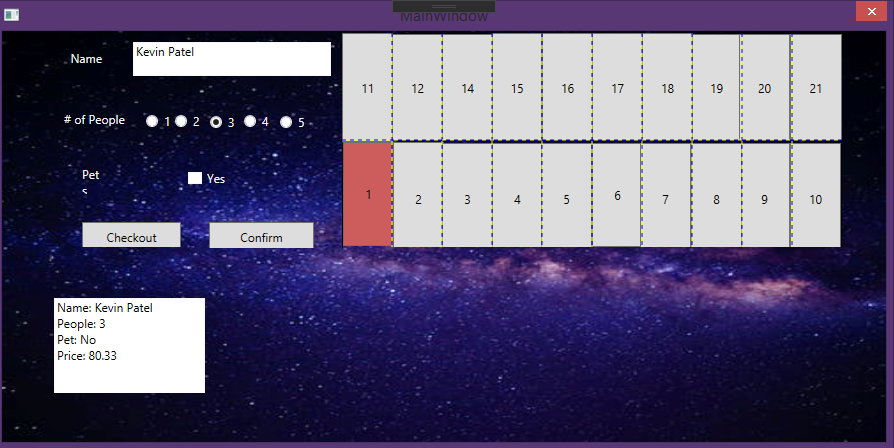
\includegraphics[height=250px, width=350px]{Main.png}
\caption{Main window of the program}
\label{Interface}
\end{figure}


\section{Project Timeline}
8/27/2019\\

A large portion of our time spent on this project was on design. To be honest, too much time was spent on the design. It wasn't until, two months in, that we started the actual coding of the project, that the design fell into place all on its own. \\
\newline 11/08/2019 \\

Within two days, we had moved past the design and delved into the requirements. First came the buttons themselves. Each button needed to act separately from the others, so it took over a month to manage everything that needed to happen upon button clicks. Some of these issues were color changes, form population, and a note system. \\
\newline 11/10/2019 \\

This last month has been committed to polishing and trying to learn a database. We eventually gave up on the database and will store all information as notes. \\
\newline 12/3/2019

\section{Project Structure}
By the project's culmination, it turned into a day to day system to manage availability of rooms for the hotel. It has a working GUI, and upon filling in the information about reservation, it will mark the room unavailable with a color change. There is another button that will change it back to available. 

All information is stored in a display box for notes, in lieu of a database. We realized there is no point since they have no rewards system in place at the hotel yet. 

\subsection{UML Outline}

\begin{figure}[ht!]
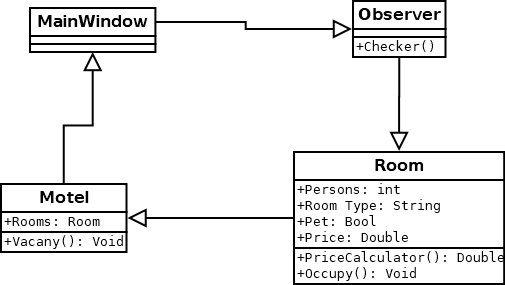
\includegraphics[height=250px, width=350px]{uml.png}
\caption{Diagram of the program's programming structure.}
\label{UML}
\end{figure}



\subsection{Design Patterns Used}
The decorator design pattern was used on buttons. Upon another button's clicking, a separate button will change color based on what the button action is doing.
The Observer Patter is also being used to constantly be looking at the rooms current state to see weather it is filled when clicked on or occupied and to appropriately show the proper results.


\section{Results}
By the end of the project, our program currently is able to handle the day-to-day management of rooms at the Stone Brook Inn, where occupied rooms are highlighted in red and the unoccupied rooms will remain their beginning grey color, also the price calculation will be handled by the system once all necessary fields are entered. 

\subsection{Future Work}
In the future, implementing a database to hold persistent data as well as and easy way to configure prices and other options within the software are to be added as well as integrating an API to pull reservations from online sites that offer online reservations, or perhaps create a website to handle that for the hotel itself. 






\end{document}